\chapter{Consignes de présentation}
\label{chap:consignes}

Vous venez de télécharger la classe personnalisée LaTeX AMU pour les thèses de doctorat de l'université d'Aix-Marseille.
Certains éléments doivent obligatoirement être utilisés:
\\


\begin{figure}[h!tbp]
	%\vspace{0.5cm}
	\centering
	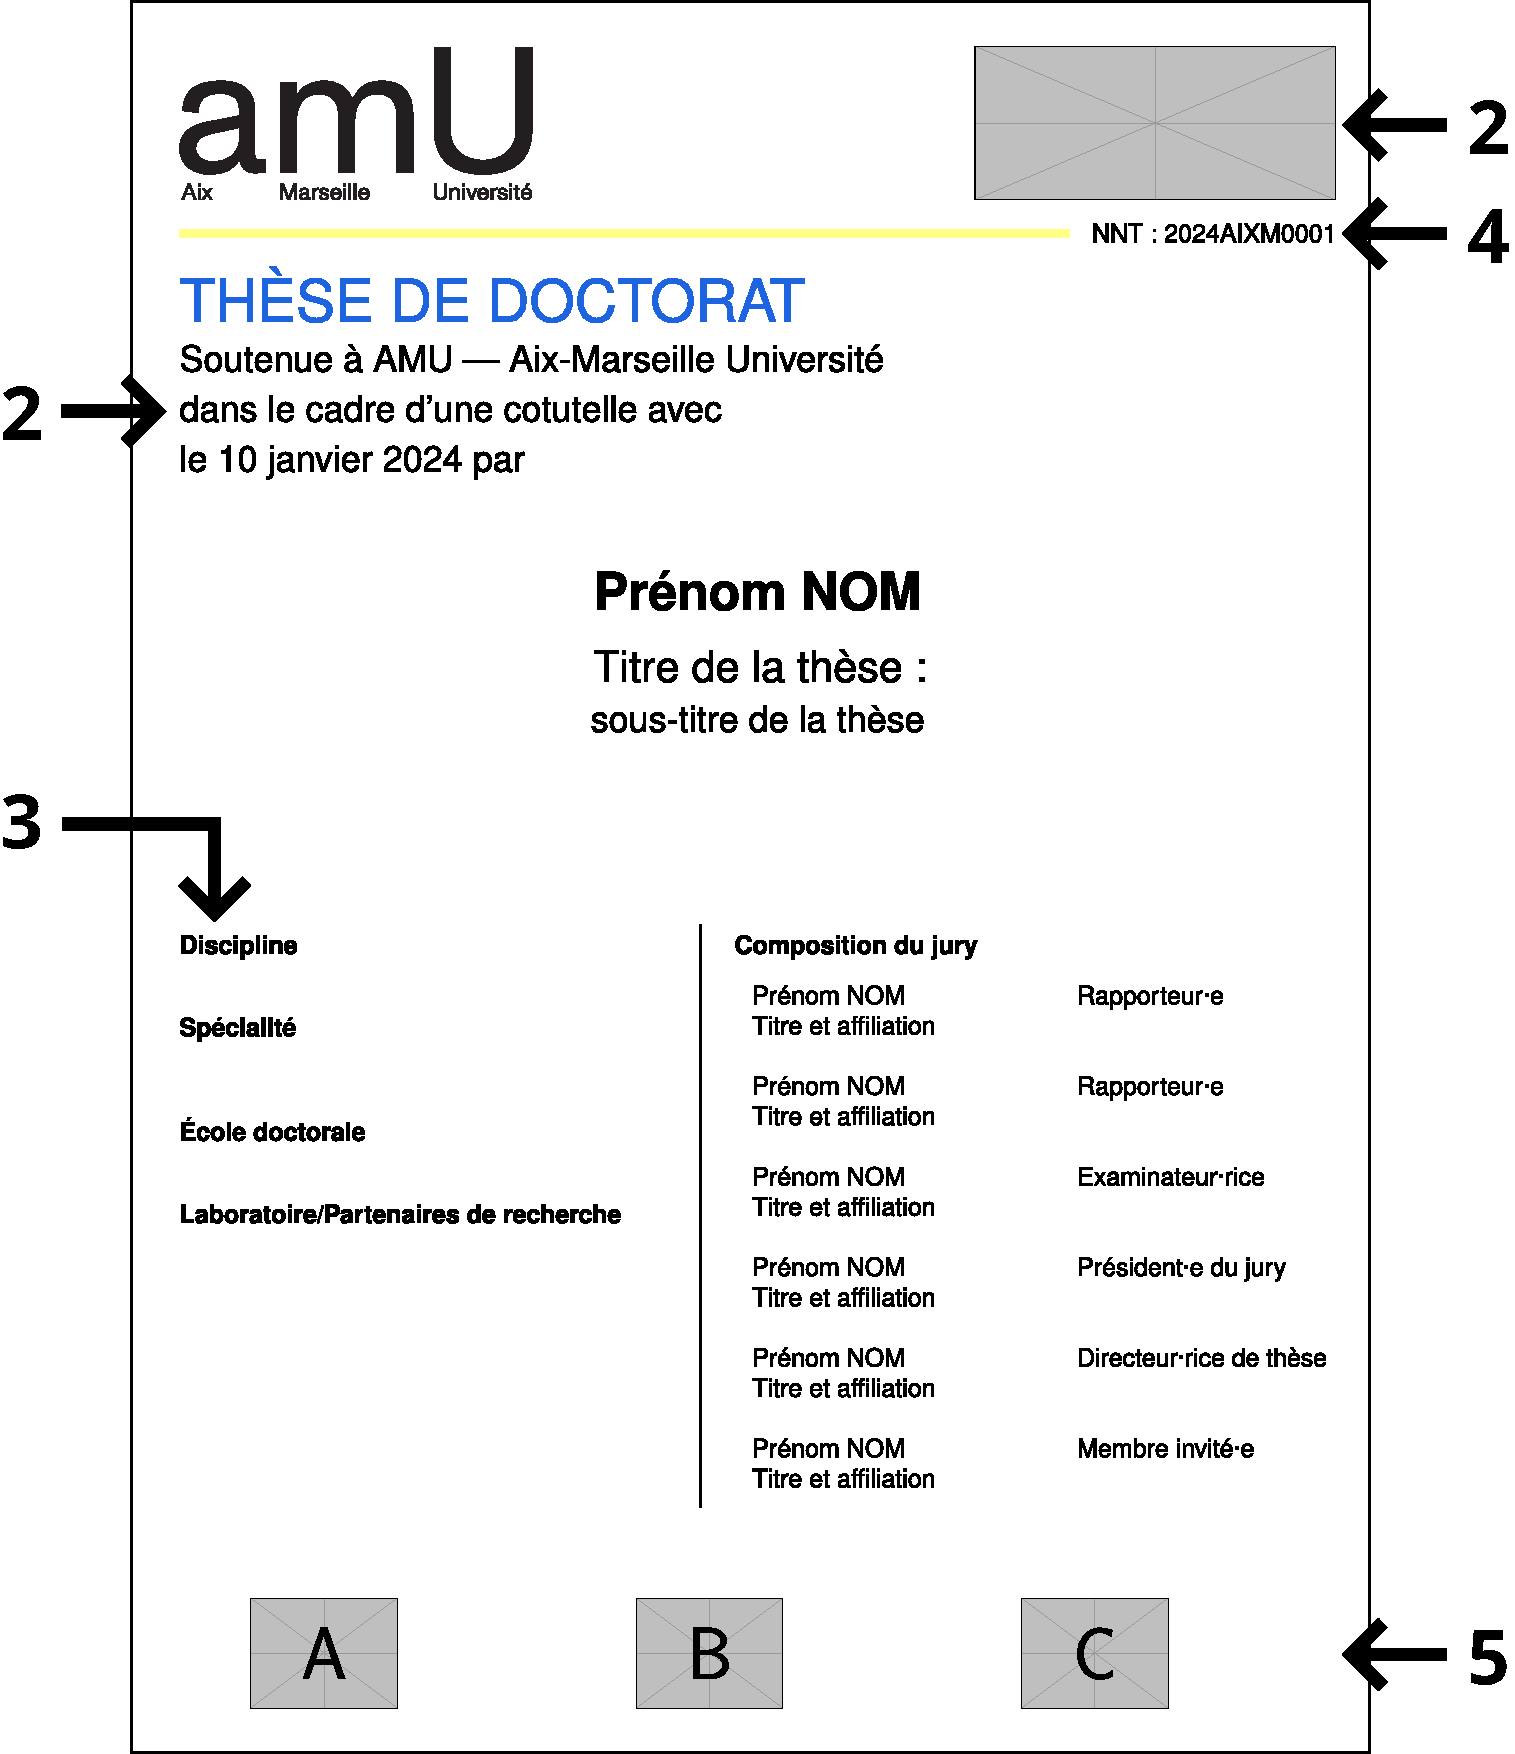
\includegraphics[width=0.8\textwidth]{titre.pdf}
\end{figure}

\begin{enumerate}
	\item La page de titre des thèses AMU: elle est rédigée en langue française avec la police Titillium, disponible avec le modèle LaTeX AMU aux formats TTF et TFM, selon la charte graphique AMU.
	\item En cas de cotutelle internationale, le logo de l’établissement partenaire doit apparaître en haut à droite de la page de titre;
	\item La composition du jury, l’école doctorale, la discipline et la spécialité (le cas échéant) doivent être conformes au formulaire ADUM de demande de soutenance de thèse;
	\item Le numéro national de thèse (NNT) doit être apposé sur la page de titre;
	\item Le cas échéant, les logos d’institutions ou d’unité de recherche partenaires peuvent être ajoutés en bas de la page de titre;
	\item La page \nameref{chap:affidavit}: selon la langue utilisée pour la rédaction de de votre thèse, opter pour la version en français ou en anglais, puis la compléter, la dater et la signer;
	\item La page \nameref{chap:publications} réalisées au cours de votre projet de thèse ;
	\item Les pages \nameref{chap:resume} en français et \nameref{chap:abstract} en anglais: chaque résumé ne doit pas dépasser 4000 caractères;
\end{enumerate}

Selon vos besoins, vous pouvez ajouter les éléments suivants: sommaire et/ou table des matières, liste des figures, liste des tableaux, liste des acronymes, glossaire, index, nomenclature…

Pour le corps de votre thèse, si votre école doctorale ne vous donne pas de consignes plus précises, vous pouvez utiliser les styles établis dans ce modèle ou vos propres styles en suivant ces recommandations:
\begin{itemize}
	\item Police neutre : Il est conseillé d'utiliser une police serif standard pour le texte et une police sans-serif standard pour les titres;
	\item Géométrie : paper=a4, fontsize=12pt, DIV=12;
	\item Interligne simple;
	\item Texte justifié.
\end{itemize}

\begin{figure}[h!tbp]
	%\vspace{0.5cm}
	\centering
	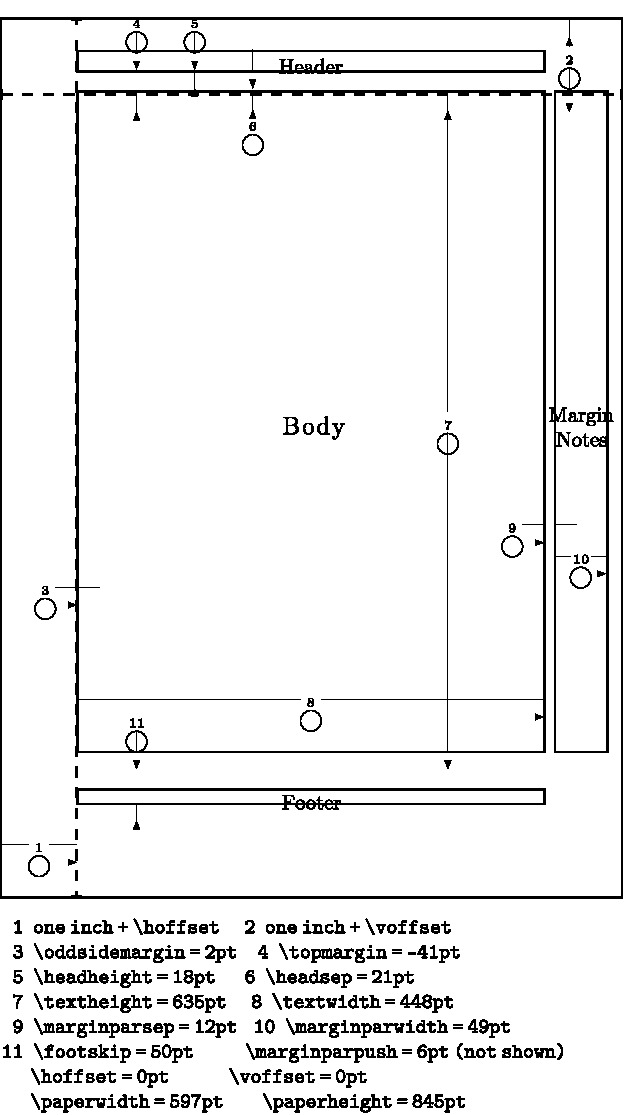
\includegraphics[width=0.3\textwidth]{geometry.pdf}
\end{figure}


Votre thèse devra être déposée en ligne en format PDF version 1.5 minimum sur \href{https://www.adum.fr/}{adum.fr}.


